\chapteropen{Chapter 11: Model-View-Controller}{chapter-11}
\markboth{Ch. 11 | MVC}{}


\begin{studycolumns}
\vspace{0pt}
\begin{eli5box}One spreadsheet Model can feed a table and chart. Controllers interpret input; a Model change notifies Views so they refresh consistently.\end{eli5box}
\textbf{Answer check:} Trace input, Model update, notification and View refresh. MVC is triangular; it can coexist with layered services/\allowbreak{}persistence.
\subsection*{11.1 The problem MVC solves}
\sectionlabel{h-111-the-problem-mvc-solves}
Use MVC for interactive systems with changing input/\allowbreak{}display behaviour and multiple synchronised views of shared information. It separates presentation and interaction from core rules/\allowbreak{}data.
\end{studycolumns}

\subsection*{11.2 Components}
\sectionlabel{h-112-components}

{\fontsize{9}{11}\selectfont
\begin{longtable}{L{\dimexpr 0.15756\linewidth-5.04pt\relax}L{\dimexpr 0.46161\linewidth-14.77pt\relax}L{\dimexpr 0.17616\linewidth-5.64pt\relax}L{\dimexpr 0.20468\linewidth-6.55pt\relax}}
\toprule
\rowcolor{ice}\textbf{Component} & \textbf{Responsibility} & \textbf{Stereotype} & \textbf{Example} \\
\midrule\endfirsthead
\toprule\rowcolor{ice}\textbf{Component} & \textbf{Responsibility} & \textbf{Stereotype} & \textbf{Example} \\
\midrule\endhead
\multicolumn{4}{r}{\scriptsize Continued on next page}\\\endfoot
\bottomrule\endlastfoot
\textbf{Model} & Contains the \textbf{processing (operations) and the data} & \guillemotleft{}control\guillemotright{} + \guillemotleft{}entity\guillemotright{} & \code{Work\allowbreak{}Sheet}, \code{Sheet\allowbreak{}Manager} \\
\textbf{View} & Defines and manages \textbf{how data is presented}; each View provides a specific presentation of the same Model; each View \textbf{observes} the Model & \guillemotleft{}boundary\guillemotright{} & \code{Line\allowbreak{}Chart}, \code{Bar\allowbreak{}Chart} \\
\textbf{Controller} & Manages \textbf{user interaction}: captures input (mouse clicks, key presses) and passes interactions to View and Model; each View is associated with a Controller; user interacts \textbf{solely through Controllers} & \guillemotleft{}boundary\guillemotright{}/\allowbreak{}\guillemotleft{}control\guillemotright{} & \code{Edit\allowbreak{}WS}, \code{Edit\allowbreak{}WSCtrler} \\
\end{longtable}
}

\subsection*{11.3 The triangular structure (know the arrows by heart)}
\sectionlabel{h-113-the-triangular-structure-know-the-arrows-by-heart}

\par\smallskip\noindent\begin{minipage}{\linewidth}\centering
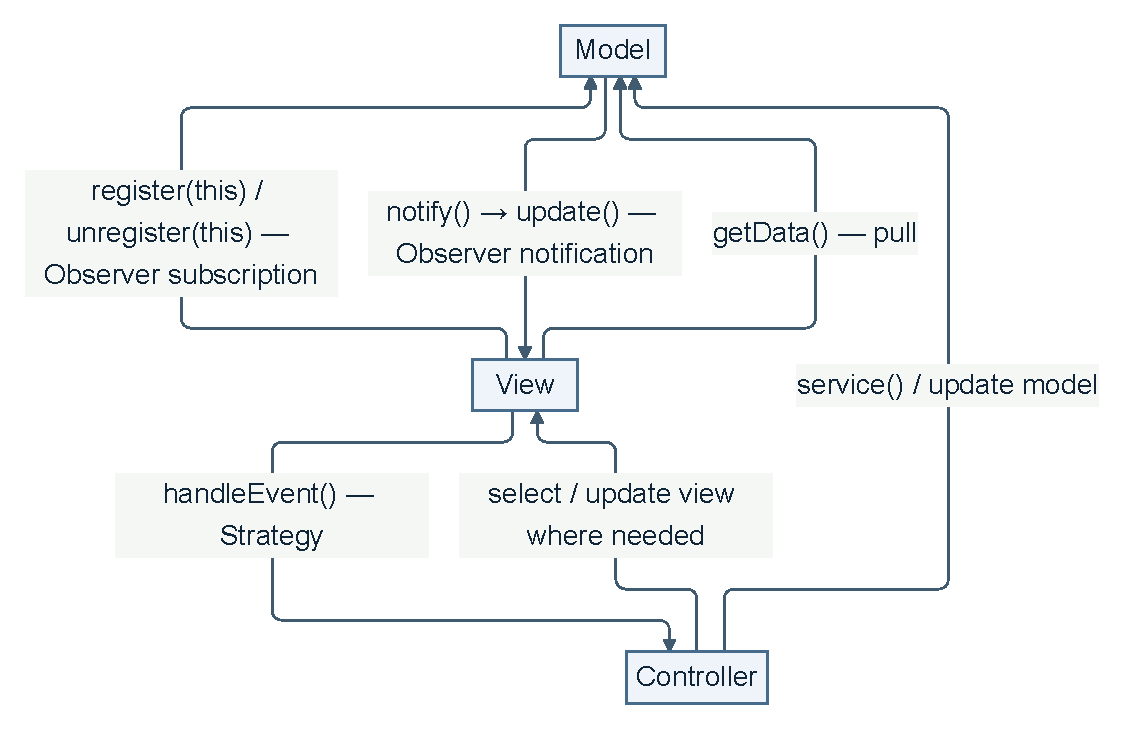
\includegraphics[width=331.20pt]{images/fig-032.pdf}
\captionof{figure}{11.3 The triangular structure (know the arrows by heart)}\end{minipage}\par\smallskip

\textbf{Arrow check:} View registers with Model; Controller invokes Model services; Model notifies subscribed Views; Views pull data and redraw. A subscribed Controller may also receive Model notifications (L15 pp. 22, 25). Observing the Model is different from observing the Controller.

\subsection*{11.4 Which patterns live inside MVC}
\sectionlabel{h-114-which-patterns-live-inside-mvc}

{\fontsize{9}{11}\selectfont
\begin{longtable}{L{\dimexpr 0.34699\linewidth-8.33pt\relax}L{\dimexpr 0.23017\linewidth-5.52pt\relax}L{\dimexpr 0.42284\linewidth-10.15pt\relax}}
\toprule
\rowcolor{ice}\textbf{Relationship} & \textbf{Pattern} & \textbf{Why} \\
\midrule\endfirsthead
\toprule\rowcolor{ice}\textbf{Relationship} & \textbf{Pattern} & \textbf{Why} \\
\midrule\endhead
\multicolumn{3}{r}{\scriptsize Continued on next page}\\\endfoot
\bottomrule\endlastfoot
\textbf{View \ensuremath{\leftrightarrow} Model; subscribed Controller \ensuremath{\leftrightarrow} Model} & \textbf{Observer} & Multiple views, loose coupling, automatic update \\
\textbf{View \ensuremath{\leftrightarrow} Controller} & \textbf{Strategy} & View delegates interface behaviour; controller swappable \ensuremath{\rightarrow} different responses to input; also View \ensuremath{\leftrightarrow} Look \& Feel \\
\textbf{Controller creation /\allowbreak{} Look \& Feel} & \textbf{Abstract Factory} & Create a controller or LAF for a view \\
\textbf{Nested views} & \textbf{Composite} & Panel contains Button; nested Panels \\
\textbf{Extra UI functionality (scrolling)} & \textbf{Decorator} & Attach additional UI functionality to a view \\
\textbf{Undo/\allowbreak{}redo of user actions} & \textbf{Command} & Support undo/\allowbreak{}redo \\
\end{longtable}
}

\begin{studycolumns}
\vspace{0pt}
\subsection*{11.5 Why MVC over plain layering (the exam argument)}
\sectionlabel{h-115-why-mvc-over-plain-layering-the-exam-argument}
\par\needspace{65pt}\phantomsection\label{answer-mvc}
\textbf{Template M --- MVC alternative:} map case state/\allowbreak{}rules to Model, presentations to Views and input handling to Controllers. Use Observer for consistent refresh; Strategy separates input/\allowbreak{}look-and-feel variation; Abstract Factory creates related UI objects. Benefits: multiple-view consistency, separate UI/\allowbreak{}domain change, testability. Costs: notification/\allowbreak{}lifecycle and multi-artifact complexity. It avoids delayed/\allowbreak{}excessive polling and concrete view-to-view callbacks; layering can remain underneath.
\subsection*{11.6 Pros /\allowbreak{} cons}
\sectionlabel{h-116-pros--cons}
\begin{referenceentries}
\textit{\textbf{Pros} / \textbf{Cons}}\par\smallskip
\noindent \textbf{Pros:} \textbf{Simultaneous development} --- multiple views per model; models can have multiple views\par
\noindent \textbf{Cons:} \textbf{Code navigability} and a pronounced \textbf{learning curve}\par\smallskip
\noindent \textbf{Pros:} \textbf{High cohesion} --- related actions grouped on a controller; views for a model grouped\par
\noindent \textbf{Cons:} Framework navigation is complex: new layers of abstraction, users must adapt to MVC's decomposition criteria\par\smallskip
\noindent \textbf{Pros:} \textbf{Low coupling} among models, views and controllers\par
\noindent \textbf{Cons:} \textbf{Multi-artifact consistency} --- one logical change touches three artefacts\par\smallskip
\end{referenceentries}\textbf{Traps:} MVC is not three deployment tiers. Its Controller is not automatically the analysis control stereotype: the course puts View/\allowbreak{}Controller in presentation boundaries, and entities plus business controls in Model. Controller updates Model; Model notifies subscribers; Views pull data and redraw.
\end{studycolumns}
